\section{Optimal Control of Pitch/Travel with Feedback (LQ)}\label{sec:prob3}
You are as mentioned welcome to use the figures from the assignment text if you want to (cite the source!). You can also draw your own (cite the source if it is heavily based on someone else's.). Figure~\ref{fig:layers_openloop} was created quickly with Ipe. Inkscape is a good alternative for more advanced illustrations. Some people prefer the Latex package TikZ (\url{http://texample.net/tikz/examples/}), but this takes a little effort to learn.

\begin{figure}[tp]
	\centering
		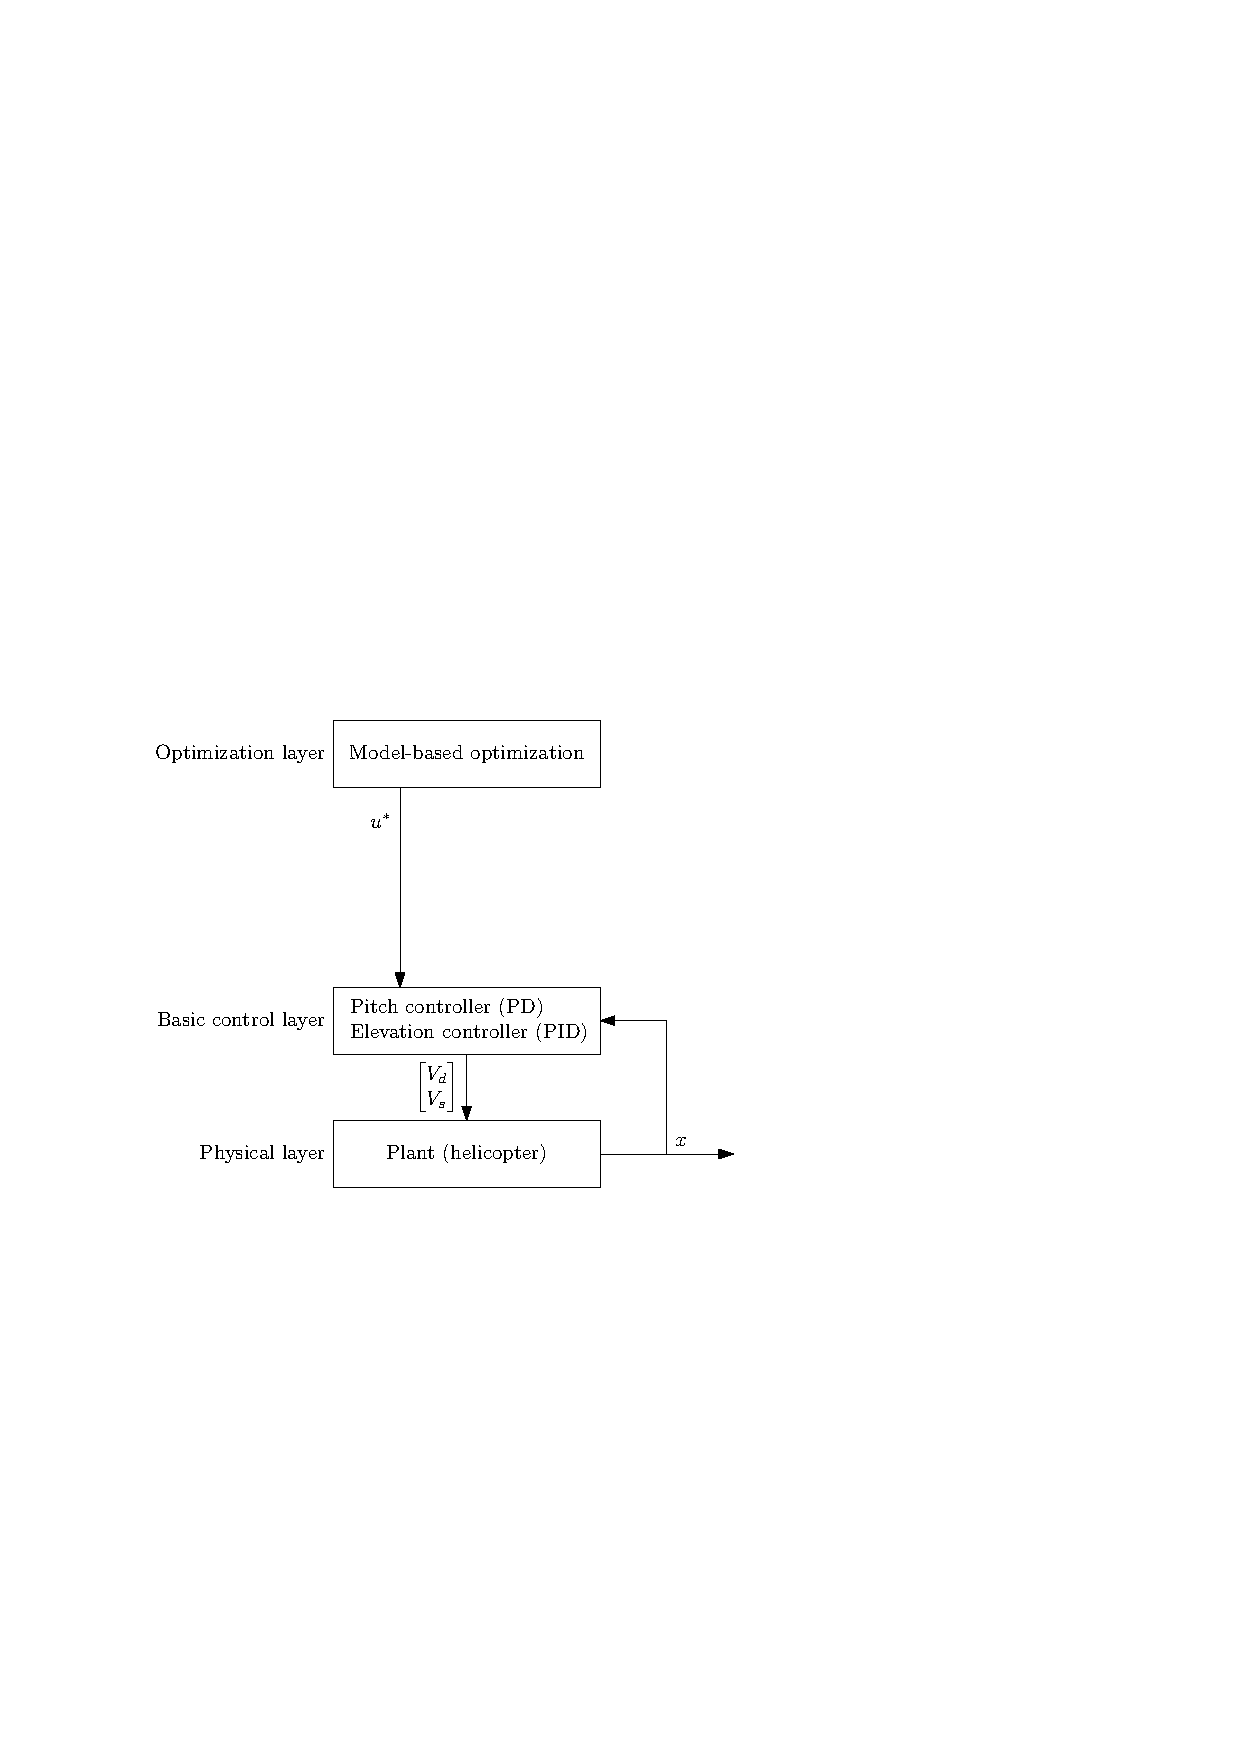
\includegraphics[width=1.00\textwidth]{figures/layers_openloop.pdf}
	\caption{A figure created with Ipe.}
	\label{fig:layers_openloop}
\end{figure}

Here is a matrix equation you can use as a template:
\begin{equation}
\begin{bmatrix}
 1 &  0 &  0 & 0 & -b &  0 &  0 &  0 \\
-a &  1 &  0 & 0 &  0 & -b &  0 &  0 \\
 0 & -a &  1 & 0 &  0 &  0 & -b &  0 \\
 0 &  0 & -a & 1 &  0 &  0 &  0 & -b                                
\end{bmatrix}
\begin{bmatrix} x_1 \\ x_2 \\ x_3 \\ x_4 \\ u_0 \\ u_1 \\ u_2 \\ u_3 \end{bmatrix}
=
\begin{bmatrix}
ax_0 \\ 0 \\ 0 \\ 0      
\end{bmatrix}
\end{equation}